\documentclass[twocolumn,10pt]{article}
\title{Slicing 3D solids}
\setlength{\columnsep}{20pt} 
\usepackage{amsmath,hyperref,cancel,graphicx}
 \def\shrinkfactor{0.55}
 \usepackage[margin=1.5cm]{geometry}
\usepackage[usenames,dvipsnames]{color}
 
 \newcommand{\blue}[1]{{\color{Blue}#1}} 
 \newcommand{\purple}[1]{{\color{Purple}#1}} 
 \newcommand{\red}[1]{{\color{Red}#1}} 
 \newcommand{\green}[1]{{\color{Green}#1}} 
 \newcommand{\gray}[1]{{\color{Gray}#1}} 
  \newcommand{\pink}[1]{{\color{Magenta}#1}}   


\begin{document}
\maketitle



\section{\href{https://www.khanacademy.org/devadmin/content/items/x141c0caeea18da08}{x141c0caeea18da08}}

\noindent
The figure below shows a pyramid with a square base. The height of the pyramid is equal to the side of its base. 

**Which two dimensional shape describes the shape of a vertical slice through the pyramid that does not pass through the center?**  


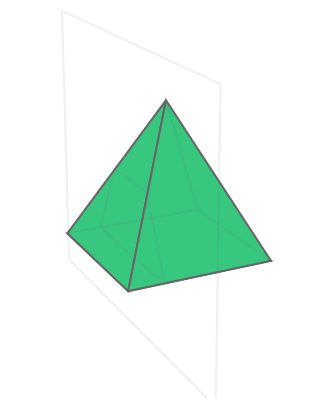
\includegraphics[scale=\shrinkfactor]{figures/9a89f6932a0ccb7754b5e179979be09a7382f1eb.png}

\paragraph{Ans} 

\fbox{ 
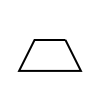
\includegraphics[scale=\shrinkfactor]{figures/462dbf19e63d9954ed7a531f7ea0e2b0379d9bb9.png}

}

 
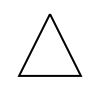
\includegraphics[scale=\shrinkfactor]{figures/d443e0deb4dc18ef30fbf9139d310266f460b66b.png}


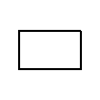
\includegraphics[scale=\shrinkfactor]{figures/0e5042b475e0847d67b74c0482f8e8173f798656.png}


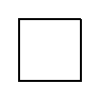
\includegraphics[scale=\shrinkfactor]{figures/4b59a0ece6acc7c19c389e1de534d1df93bf1169.png}



\paragraph{Hint 1}The slice cuts through the pyramid vertically, but not through the center.

\paragraph{Hint 2}The pyramid looks like a triangle when sliced vertically through its center.

When the pyramid is sliced vertically not passing through it looks like a trapezoid.

\paragraph{Hint 3}The shape that we'll see in a vertical slice through the pyramid is an isosceles trapezoid.  

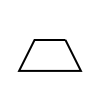
\includegraphics[scale=\shrinkfactor]{figures/462dbf19e63d9954ed7a531f7ea0e2b0379d9bb9.png}




\medskip
\noindent
\textbf{Tags:} {\footnotesize Slicing 3d figures.solid to section, CC.7.G.A.3, SB.7.1.E.4.SR}\\
\textbf{Version:} 67223d20.. 2013-10-02
\smallskip\hrule





\section{\href{https://www.khanacademy.org/devadmin/content/items/x209d34a33212eb67}{x209d34a33212eb67}}

\noindent
Taking a horizontal slice through a three dimensional solid produces the following two dimensional shape.

**When sliced horizontally, which of the following solids would produce this two dimensional shape?**   

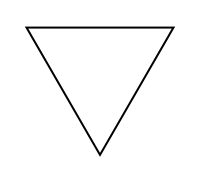
\includegraphics[scale=\shrinkfactor]{figures/788a8b56b0b7607b1ee5b54e7626cf4b802e373f.png} 


\paragraph{Ans} 

\fbox{ 

\includegraphics[scale=\shrinkfactor]{figures/df7e52cb3a541015199076ff457ee6bdda3a663c.png}

}

 
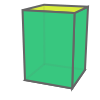
\includegraphics[scale=\shrinkfactor]{figures/5f94871e71f674049268d58ac56b3de4dfa3a3ba.png}



\includegraphics[scale=\shrinkfactor]{figures/714aa411c23dfb02df032183d703d78050ecb5ae.png}


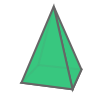
\includegraphics[scale=\shrinkfactor]{figures/8e0bce39d089e690c82fd2275ed9e00339fd8202.png}



\paragraph{Hint 1}The shape we see in the two dimensional slice is a triangle. Therefore, the solid which was sliced must have a triangular base. 

\paragraph{Hint 2}Which of the solids in the choices has a triangular base?

\paragraph{Hint 3}Only the right prism with a triangular base would produce a triangle when sliced horizontally.



\includegraphics[scale=\shrinkfactor]{figures/df7e52cb3a541015199076ff457ee6bdda3a663c.png}



\medskip
\noindent
\textbf{Tags:} {\footnotesize Slicing 3d figures.section to solid, CC.7.G.A.3, SB.7.1.E.4.SR}\\
\textbf{Version:} 7b9b9e07.. 2013-10-01
\smallskip\hrule





\section{\href{https://www.khanacademy.org/devadmin/content/items/x2e7aee12e3895c4c}{x2e7aee12e3895c4c}}

\noindent
A vertical slice through a three dimensional solid produces a two dimensional shape.

**When sliced vertically, which of the following solids would produce this two dimensional shape?**   

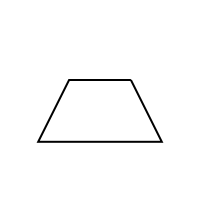
\includegraphics[scale=\shrinkfactor]{figures/9a01e5fee86b7569b86f7e8f116595d328925a8c.png} 


\paragraph{Ans} 


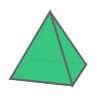
\includegraphics[scale=\shrinkfactor]{figures/49b99cca0c4e580ceaef3d4fd5842ea463191ce8.png}


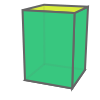
\includegraphics[scale=\shrinkfactor]{figures/5f94871e71f674049268d58ac56b3de4dfa3a3ba.png}



\includegraphics[scale=\shrinkfactor]{figures/714aa411c23dfb02df032183d703d78050ecb5ae.png}

\fbox{ 

\includegraphics[scale=\shrinkfactor]{figures/df7e52cb3a541015199076ff457ee6bdda3a663c.png}

}

 

\paragraph{Hint 1}The shape we see in the two dimensional slice is an isosceles trapezoid. It is a trapezoid because it has two parallel sides and it is isosceles because its left side looks like the mirror image of the right side, like an isosceles triangle.

\paragraph{Hint 2}Which of the solids in the choices would produce a shape with sloping sides when sliced vertically?

\paragraph{Hint 3}The triangular, square, and pentagonal prisms all have vertical sides so slicing them vertically cannot produce a shape with sloping sides.

\paragraph{Hint 4}Only the pyramid with would a two dimensional shape with sloping sides.


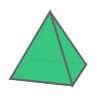
\includegraphics[scale=\shrinkfactor]{figures/49b99cca0c4e580ceaef3d4fd5842ea463191ce8.png}

To produce an isosceles trapezoid, slice the pyramid using a slice that does not pass through the center.


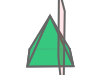
\includegraphics[scale=\shrinkfactor]{figures/5c4f5d18cffbd9888619838aea65c59f3f17f1d0.png}



\medskip
\noindent
\textbf{Tags:} {\footnotesize Slicing 3d figures.section to solid, CC.7.G.A.3, SB.7.1.E.4.SR}\\
\textbf{Version:} 8b12cc53.. 2013-10-07
\smallskip\hrule





\section{\href{https://www.khanacademy.org/devadmin/content/items/x352783df3e596cf8}{x352783df3e596cf8}}

\noindent
The figure below shows a pyramid with a square base. The height of the pyramid is equal to the side of its base. 

**Which two dimensional shapes can be obtained as  horizontal or vertical slices through the pyramid?**  


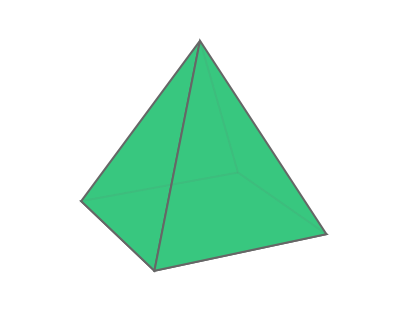
\includegraphics[scale=\shrinkfactor]{figures/1d9b248d33b33b47f6b0bcbfae27cf51e2c208c7.png}

[[? categorization 1]]

\paragraph{Ans} Drag and drop each card into the appropriate category. 

\paragraph{Hint 1}The pyramid looks like a triangle when sliced vertically through its center.  

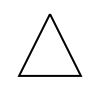
\includegraphics[scale=\shrinkfactor]{figures/d443e0deb4dc18ef30fbf9139d310266f460b66b.png}

\paragraph{Hint 2}When the pyramid is sliced vertically not passing through the center, the slice has the shape of an isosceles trapezoid.   

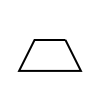
\includegraphics[scale=\shrinkfactor]{figures/462dbf19e63d9954ed7a531f7ea0e2b0379d9bb9.png}

\paragraph{Hint 3}The shape of a horizontal slice through the pyramid looks like a square.  

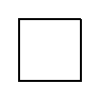
\includegraphics[scale=\shrinkfactor]{figures/4b59a0ece6acc7c19c389e1de534d1df93bf1169.png}

\paragraph{Hint 4}It is not possible to obtain the other shapes by slicing the pyramid**.**



\medskip
\noindent
\textbf{Tags:} {\footnotesize Slicing 3d figures.solid to section, CC.7.G.A.3, SB.7.1.E.4.SR}\\
\textbf{Version:} 5dea6666.. 2013-10-02
\smallskip\hrule





\section{\href{https://www.khanacademy.org/devadmin/content/items/x462b5e87a5ace1db}{x462b5e87a5ace1db}}

\noindent
The figure below shows a cube with side length $3$.   

**Draw the shape you will see if you take a horizontal slice through the cube.**


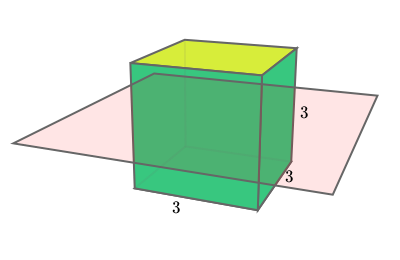
\includegraphics[scale=\shrinkfactor]{figures/f0b7654c0b53908504fb120f51f2b50f3f8fd955.png}

[[? interactive-graph 1]]




\paragraph{Ans} Move the points to draw the shape. 

\paragraph{Hint 1}The slice cuts through the cube horizontally, so the shape we'll see in the slice is the same as the shape of the base of the cube.

\paragraph{Hint 2}Since the cube case side length $3$, the base of the cube has the shape of a $3 \times 3$ square. 


\paragraph{Hint 3}The shape of the horizontal slice through the cube is a $3 \times 3$ square:  

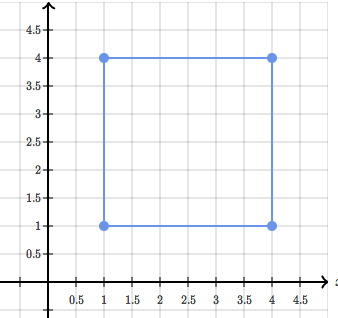
\includegraphics[scale=\shrinkfactor]{figures/cb2ed34a4e2c927dc5486305caad138960eaf2e0.png}



\medskip
\noindent
\textbf{Tags:} {\footnotesize Slicing 3d figures.draw section, CC.7.G.A.3, SB.7.1.E.4.SR}\\
\textbf{Version:} 61df89ad.. 2013-10-02
\smallskip\hrule





\section{\href{https://www.khanacademy.org/devadmin/content/items/x6b70eb108befb974}{x6b70eb108befb974}}

\noindent
The figure below shows prism whose base is a $3\times 3$ square and whose height is $6$.   

**Draw the shape you will see if you take a vertical slice through the prism.**


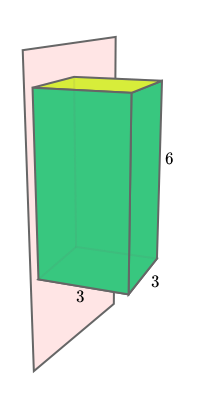
\includegraphics[scale=\shrinkfactor]{figures/94bf14f4775048a20e633abd42558d8e108ecfab.png}

[[? interactive-graph 1]] 

\paragraph{Ans} Move the points to draw the shape. 

\paragraph{Hint 1}The slice cuts through the prism vertically, so the shape we'll see in the slice is the same as the shape of the side of the prism.

\paragraph{Hint 2}The side of the prism is rectangle with base $3$ and height $6$.

\paragraph{Hint 3}The shape of the vertical slice through the prism is a $3 \times 6$ rectangle:   

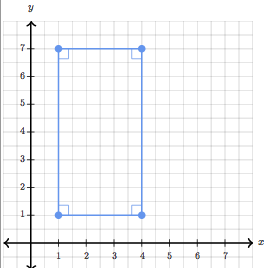
\includegraphics[scale=\shrinkfactor]{figures/afdbf1f1510de1b384cf8ec99b6646737b06944a.png}



\medskip
\noindent
\textbf{Tags:} {\footnotesize Slicing 3d figures.draw section, CC.7.G.A.3, SB.7.1.E.4.SR}\\
\textbf{Version:} 016ad1ca.. 2013-10-02
\smallskip\hrule





\section{\href{https://www.khanacademy.org/devadmin/content/items/x72bb801397b54d5e}{x72bb801397b54d5e}}

\noindent
The figure below shows a right rectangular pyramid whose base is a square.

**Which two dimensional shape describes the shape of a horizontal slice through the pyramid?**  


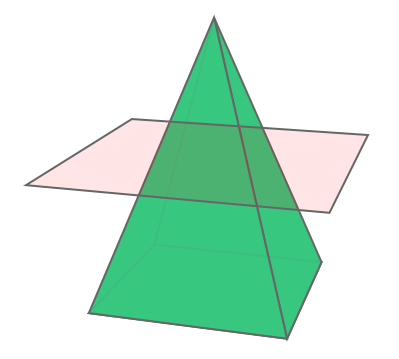
\includegraphics[scale=\shrinkfactor]{figures/3f0ba787b169725c8c4c74a3017b4210d7a511f5.png}

\paragraph{Ans} 


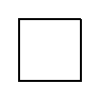
\includegraphics[scale=\shrinkfactor]{figures/4b59a0ece6acc7c19c389e1de534d1df93bf1169.png}


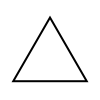
\includegraphics[scale=\shrinkfactor]{figures/15c855a8a232e6c1873c5f46769050a9c13051b8.png}


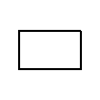
\includegraphics[scale=\shrinkfactor]{figures/0e5042b475e0847d67b74c0482f8e8173f798656.png}

\fbox{ 
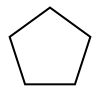
\includegraphics[scale=\shrinkfactor]{figures/498a6b09730fdba2360826c138eeee142e8cccc1.png}

}

 

\paragraph{Hint 1}The slice cuts through the pyramid horizontally so the shape we'll see in the slice is the same as the shape of the base of the pyramid.

\paragraph{Hint 2}Since the shape of the pyramid's base is a square, the shape of the horizontal slice is also a square.

\paragraph{Hint 3}The shape that we'll see in a horizontal slice through the pyramid is a square.  

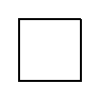
\includegraphics[scale=\shrinkfactor]{figures/4b59a0ece6acc7c19c389e1de534d1df93bf1169.png}



\medskip
\noindent
\textbf{Tags:} {\footnotesize Slicing 3d figures.solid to section, CC.7.G.A.3, SB.7.1.E.4.SR}\\
\textbf{Version:} 578cd0e2.. 2013-10-01
\smallskip\hrule





\section{\href{https://www.khanacademy.org/devadmin/content/items/x7b7f9e81dc7e0cea}{x7b7f9e81dc7e0cea}}

\noindent
The figure below shows a right rectangular prism whose base is a pentagon.

**Which two dimensional shape describes the shape of a horizontal slice through the prism?**  


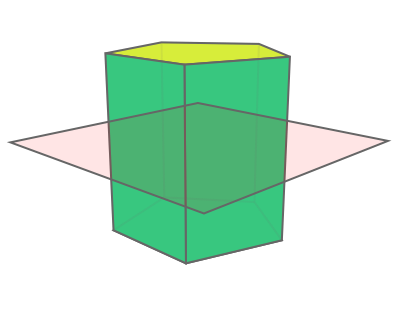
\includegraphics[scale=\shrinkfactor]{figures/fe9352beb31c400cf0f7b64a1efed2b946206cc4.png}

\paragraph{Ans} 

\fbox{ 
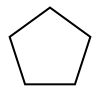
\includegraphics[scale=\shrinkfactor]{figures/498a6b09730fdba2360826c138eeee142e8cccc1.png}

}

 
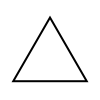
\includegraphics[scale=\shrinkfactor]{figures/15c855a8a232e6c1873c5f46769050a9c13051b8.png}


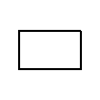
\includegraphics[scale=\shrinkfactor]{figures/0e5042b475e0847d67b74c0482f8e8173f798656.png}


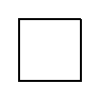
\includegraphics[scale=\shrinkfactor]{figures/4b59a0ece6acc7c19c389e1de534d1df93bf1169.png}



\paragraph{Hint 1}The slice cuts through the prism horizontally so the shape we'll see in the slice is the same as the shape of the base of the prism.

\paragraph{Hint 2}Since the shape of the prism is a pentagon, the shape of the horizontal slice is also a pentagon.

\paragraph{Hint 3}The shape that we'll see in a horizontal slice through the prism is a pentagon.  

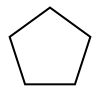
\includegraphics[scale=\shrinkfactor]{figures/498a6b09730fdba2360826c138eeee142e8cccc1.png}



\medskip
\noindent
\textbf{Tags:} {\footnotesize Slicing 3d figures.solid to section, CC.7.G.A.3, SB.7.1.E.4.SR}\\
\textbf{Version:} ca4dc10e.. 2013-10-01
\smallskip\hrule





\section{\href{https://www.khanacademy.org/devadmin/content/items/x80dc1341b9007790}{x80dc1341b9007790}}

\noindent
The figure below shows a right rectangular prism with base $2 \times 2$ and height $4$. 

**Which two dimensional shape describes the shape of a horizontal slice through the prism?**  


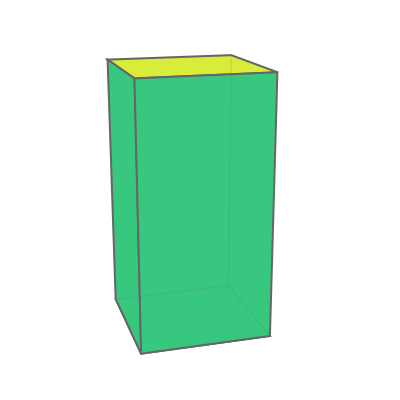
\includegraphics[scale=\shrinkfactor]{figures/5fc465f62d5e1338260e3fddfd32bff967dffbdf.png}

\paragraph{Ans} 


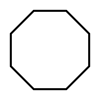
\includegraphics[scale=\shrinkfactor]{figures/7d98a99c75a84da8f748444ad7a3a8053be16a27.png}


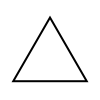
\includegraphics[scale=\shrinkfactor]{figures/15c855a8a232e6c1873c5f46769050a9c13051b8.png}


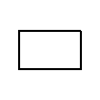
\includegraphics[scale=\shrinkfactor]{figures/0e5042b475e0847d67b74c0482f8e8173f798656.png}

\fbox{ 
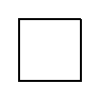
\includegraphics[scale=\shrinkfactor]{figures/4b59a0ece6acc7c19c389e1de534d1df93bf1169.png}

}

 

\paragraph{Hint 1}The slice cuts through the prism horizontally, so the shape we'll see in the slice is the same as the shape of the base of the prism.

\paragraph{Hint 2}Since the shape of the prism is a $2 \times 2$ square, the shape of the horizontal slice is also a $2 \times 2$ square.

\paragraph{Hint 3}The shape that we'll see in a horizontal slice through the prism is a square.  

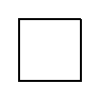
\includegraphics[scale=\shrinkfactor]{figures/4b59a0ece6acc7c19c389e1de534d1df93bf1169.png}



\medskip
\noindent
\textbf{Tags:} {\footnotesize Slicing 3d figures.solid to section, CC.7.G.A.3, SB.7.1.E.4.SR}\\
\textbf{Version:} 5538c152.. 2013-10-01
\smallskip\hrule





\section{\href{https://www.khanacademy.org/devadmin/content/items/x8bf3dcc1812f07b6}{x8bf3dcc1812f07b6}}

\noindent
A horizontal slice through a three dimensional solid produces a two dimensional shape.

**When sliced horizontally, which of the following solids would produce this two dimensional shape?**   

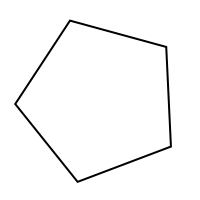
\includegraphics[scale=\shrinkfactor]{figures/f6f3d7d862af181c9db9337ad959b4868e25835c.png} 


\paragraph{Ans} 



\includegraphics[scale=\shrinkfactor]{figures/df7e52cb3a541015199076ff457ee6bdda3a663c.png}


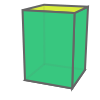
\includegraphics[scale=\shrinkfactor]{figures/5f94871e71f674049268d58ac56b3de4dfa3a3ba.png}

\fbox{ 

\includegraphics[scale=\shrinkfactor]{figures/714aa411c23dfb02df032183d703d78050ecb5ae.png}

}

 
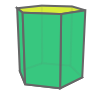
\includegraphics[scale=\shrinkfactor]{figures/994232bee673b9d41efe1aa168ac2544d5531e55.png}



\paragraph{Hint 1}The shape we see in the two dimensional slice is a pentagon.

\paragraph{Hint 2}Which of the solids in the choices would produce a pentagonal shape when sliced horizontally? 

Which of the solids has a pentagonal base?

\paragraph{Hint 3}The prism with a pentagonal base would produces a pentagonal when sliced horizontally.


\includegraphics[scale=\shrinkfactor]{figures/714aa411c23dfb02df032183d703d78050ecb5ae.png}



\medskip
\noindent
\textbf{Tags:} {\footnotesize Slicing 3d figures.section to solid, CC.7.G.A.3, SB.7.1.E.4.SR}\\
\textbf{Version:} ca3d6e14.. 2013-10-07
\smallskip\hrule





\section{\href{https://www.khanacademy.org/devadmin/content/items/xa33f179a801021da}{xa33f179a801021da}}

\noindent
The figure below shows a right rectangular prism with base $2 \times 2$ and height $4$. 

**Which two dimensional shape describes the shape of a vertical slice through the prism?**  


\includegraphics[scale=\shrinkfactor]{figures/75387eceae9780c601f242416bc9fa79e993b9b0.png}

\paragraph{Ans} 

\fbox{ 
\includegraphics[scale=\shrinkfactor]{figures/225bc3d058cebe2059fc56f78ef80b5f3e0f2da7.png}

}

 
\includegraphics[scale=\shrinkfactor]{figures/15c855a8a232e6c1873c5f46769050a9c13051b8.png}


\includegraphics[scale=\shrinkfactor]{figures/7d98a99c75a84da8f748444ad7a3a8053be16a27.png}


\includegraphics[scale=\shrinkfactor]{figures/4b59a0ece6acc7c19c389e1de534d1df93bf1169.png}



\paragraph{Hint 1}The slice cuts through the prism vertically so the shape we'll see in the slice is the same as the shape of the side of the prism.

\paragraph{Hint 2}Since the side of the prism is a $2 \times 4$ rectangle, the shape of the vertical slice is also a $2 \times 4$ rectangle.

\paragraph{Hint 3}The shape that we'll see in a vertical slice through the prism is a rectangle.   

\includegraphics[scale=\shrinkfactor]{figures/225bc3d058cebe2059fc56f78ef80b5f3e0f2da7.png}



\medskip
\noindent
\textbf{Tags:} {\footnotesize Slicing 3d figures.solid to section, CC.7.G.A.3, SB.7.1.E.4.SR}\\
\textbf{Version:} f4a02dd3.. 2013-10-02
\smallskip\hrule





\section{\href{https://www.khanacademy.org/devadmin/content/items/xddab61063efd799b}{xddab61063efd799b}}

\noindent
The figure below shows a pyramid with a square base. The height of the pyramid is equal to the side of its base. 

**Which two dimensional shape describes the shape of a vertical slice through the center of the  pyramid?**  


\includegraphics[scale=\shrinkfactor]{figures/5886f271642379937f772874924e3bcee68b664a.png}

\paragraph{Ans} 


\includegraphics[scale=\shrinkfactor]{figures/4b59a0ece6acc7c19c389e1de534d1df93bf1169.png}

\fbox{ 
\includegraphics[scale=\shrinkfactor]{figures/d443e0deb4dc18ef30fbf9139d310266f460b66b.png}

}

 
\includegraphics[scale=\shrinkfactor]{figures/0e5042b475e0847d67b74c0482f8e8173f798656.png}


\includegraphics[scale=\shrinkfactor]{figures/0245164f3f4897772e76d361f955075a80732b03.png}



\paragraph{Hint 1}The slice cuts through the pyramid vertically and passes through the center of the pyramid.

What is the shape of the pyramid when you look at it from the side?

\paragraph{Hint 2}The pyramid looks like a triangle when slices vertically through its center.

\paragraph{Hint 3}The shape that we'll see in a vertical slice through the center of the pyramid is an isosceles triangle whose height is equal to the length of its base.  

\includegraphics[scale=\shrinkfactor]{figures/d443e0deb4dc18ef30fbf9139d310266f460b66b.png}




\medskip
\noindent
\textbf{Tags:} {\footnotesize Slicing 3d figures.solid to section, CC.7.G.A.3, SB.7.1.E.4.SR}\\
\textbf{Version:} 0d6f4b87.. 2013-10-02
\smallskip\hrule



%%  Create a directory called 'figures' in latex dir and run the following command 
%  wget \
%    https://ka-perseus-graphie.s3.amazonaws.com/9a89f6932a0ccb7754b5e179979be09a7382f1eb.png \
%    https://ka-perseus-graphie.s3.amazonaws.com/462dbf19e63d9954ed7a531f7ea0e2b0379d9bb9.png \
%    https://ka-perseus-graphie.s3.amazonaws.com/d443e0deb4dc18ef30fbf9139d310266f460b66b.png \
%    https://ka-perseus-graphie.s3.amazonaws.com/0e5042b475e0847d67b74c0482f8e8173f798656.png \
%    https://ka-perseus-graphie.s3.amazonaws.com/4b59a0ece6acc7c19c389e1de534d1df93bf1169.png \
%    https://ka-perseus-graphie.s3.amazonaws.com/788a8b56b0b7607b1ee5b54e7626cf4b802e373f.png \
%    https://ka-perseus-graphie.s3.amazonaws.com/df7e52cb3a541015199076ff457ee6bdda3a663c.png \
%    https://ka-perseus-graphie.s3.amazonaws.com/5f94871e71f674049268d58ac56b3de4dfa3a3ba.png \
%    https://ka-perseus-graphie.s3.amazonaws.com/714aa411c23dfb02df032183d703d78050ecb5ae.png \
%    https://ka-perseus-graphie.s3.amazonaws.com/8e0bce39d089e690c82fd2275ed9e00339fd8202.png \
%    https://ka-perseus-graphie.s3.amazonaws.com/9a01e5fee86b7569b86f7e8f116595d328925a8c.png \
%    https://ka-perseus-graphie.s3.amazonaws.com/49b99cca0c4e580ceaef3d4fd5842ea463191ce8.png \
%    https://ka-perseus-graphie.s3.amazonaws.com/5c4f5d18cffbd9888619838aea65c59f3f17f1d0.png \
%    https://ka-perseus-graphie.s3.amazonaws.com/1d9b248d33b33b47f6b0bcbfae27cf51e2c208c7.png \
%    https://ka-perseus-graphie.s3.amazonaws.com/f0b7654c0b53908504fb120f51f2b50f3f8fd955.png \
%    https://ka-perseus-images.s3.amazonaws.com/cb2ed34a4e2c927dc5486305caad138960eaf2e0.png \
%    https://ka-perseus-graphie.s3.amazonaws.com/94bf14f4775048a20e633abd42558d8e108ecfab.png \
%    https://ka-perseus-images.s3.amazonaws.com/afdbf1f1510de1b384cf8ec99b6646737b06944a.png \
%    https://ka-perseus-graphie.s3.amazonaws.com/3f0ba787b169725c8c4c74a3017b4210d7a511f5.png \
%    https://ka-perseus-graphie.s3.amazonaws.com/15c855a8a232e6c1873c5f46769050a9c13051b8.png \
%    https://ka-perseus-graphie.s3.amazonaws.com/498a6b09730fdba2360826c138eeee142e8cccc1.png \
%    https://ka-perseus-graphie.s3.amazonaws.com/fe9352beb31c400cf0f7b64a1efed2b946206cc4.png \
%    https://ka-perseus-graphie.s3.amazonaws.com/5fc465f62d5e1338260e3fddfd32bff967dffbdf.png \
%    https://ka-perseus-graphie.s3.amazonaws.com/7d98a99c75a84da8f748444ad7a3a8053be16a27.png \
%    https://ka-perseus-graphie.s3.amazonaws.com/f6f3d7d862af181c9db9337ad959b4868e25835c.png \
%    https://ka-perseus-graphie.s3.amazonaws.com/994232bee673b9d41efe1aa168ac2544d5531e55.png \
%    https://ka-perseus-graphie.s3.amazonaws.com/75387eceae9780c601f242416bc9fa79e993b9b0.png \
%    https://ka-perseus-graphie.s3.amazonaws.com/225bc3d058cebe2059fc56f78ef80b5f3e0f2da7.png \
%    https://ka-perseus-graphie.s3.amazonaws.com/5886f271642379937f772874924e3bcee68b664a.png \
%    https://ka-perseus-graphie.s3.amazonaws.com/0245164f3f4897772e76d361f955075a80732b03.png \


\end{document}

